% Document releated
% \documentclass[12pt]{report}
%\RequirePackage[T1]{fontenc}
%\RequirePackage[utf8]{inputenc}
%\RequirePackage{environ}

\documentclass[12pt, numbers=noenddot, bibliography=totoc, headings=openright, twoside=semi]{scrbook}
\usepackage[utf8]{inputenc}
\usepackage[T1]{fontenc}
\usepackage{lmodern}
\usepackage[catalan]{babel}
\usepackage{afterpage}

% Configuration of KOMA-script
\setkomafont{dictumtext}{\itshape\small}
\setkomafont{dictumauthor}{\normalfont}
\renewcommand*\dictumwidth{0.75\linewidth}
\renewcommand*\dictumauthorformat[1]{\vspace{0.5cm}--- #1\vspace{0.25cm}}
\renewcommand*\dictumrule{}

% Table of contents depth
\setcounter{tocdepth}{2}

% Cover configuration commands
\def\title#1{\gdef\@title{#1}\gdef\thetitle{#1}}
\def\subtitle#1{\gdef\@subtitle{#1}\gdef\thesubtitle{#1}}
\def\author#1{\gdef\@author{#1}\gdef\theauthor{#1}}
\def\advisor#1{\gdef\@advisor{#1}\gdef\theadvisor{#1}}

% Graphics
\usepackage[labelsep=endash]{caption}
\usepackage{graphicx}
\usepackage{tikz}
\usepackage{newfloat}
\usepackage{subcaption}
\setlength{\abovecaptionskip}{10pt}
\setlength{\belowcaptionskip}{10pt}
\renewcommand{\thesubtable}{\roman{subtable}}
\renewcommand{\thesubfigure}{\roman{subfigure}}
\newenvironment{code}{\captionsetup{type=listing}}{}

% Symbols and Math
\usepackage{amssymb}
\usepackage{amsmath}

% Horizontal lists
\usepackage{tasks}

% Code listings
\usepackage{listings}
\lstset{
  breaklines=true,
  basicstyle=\ttfamily
}
\lstset{columns=fullflexible,basicstyle=\ttfamily}
\usepackage{minted}
%\usemintedstyle{colorful}
\setminted{breaklines=true, baselinestretch=1}
%\DeclareBoolOption{newfloat}

% References and links
\PassOptionsToPackage{hyphens}{url}\usepackage{hyperref}
\addto\extrasenglish{\renewcommand{\chapterautorefname}{Chapter}}
\providecommand*{\listingautorefname}{Listing}
\renewcommand{\lstlistingname}{Listing}
\hypersetup{hidelinks=true}
\usepackage[usestackEOL]{stackengine}

% Custom tab command
\newcommand\tab[1][10mm]{\hspace*{#1}}

% Tables configuration
\setlength{\tabcolsep}{0.6em}
{\renewcommand{\arraystretch}{1.35}

% Footnotes
\renewcommand{\thefootnote}{\textbf{\arabic{footnote}}}
\addtolength{\footnotesep}{1.5mm}
\setlength{\skip\footins}{1cm}

% Bibliography
\usepackage[
    backend=bibtex,
    style=alphabetic,
    citestyle=alphabetic
]{biblatex}
\addbibresource{references}
\nocite{*}

% Headers and footers
\usepackage{fancyhdr,lastpage}
\pagestyle{fancy}
\fancyhf{}
% \renewcommand{\chaptermark}[1]{\markboth{\MakeUppercase{\thechapter.\ #1}}{}}
\renewcommand{\headrulewidth}{0pt}
\renewcommand{\footrulewidth}{0pt}
\fancypagestyle{plain}{
\fancyhf{}
\fancyfoot[RO,LE]{\textit{\thepage}}}
% Identations and newlines
\usepackage[parfill]{parskip}
\usetikzlibrary{
    automata,calc,trees,positioning,arrows,chains,shapes.geometric,
    decorations.pathreplacing,decorations.pathmorphing,shapes,
    matrix,shapes.symbols
}
\tikzset{
    block/.style={rectangle, rounded corners, minimum height=3em, draw=black, very thick,, text centered ,text width=7.5em},
    square/.style={rectangle, draw=black, thick,, text centered},
    big_block/.style={rectangle, rounded corners, minimum height=3em, draw=black, very thick,, text centered ,text width=10em},
    bigger_block/.style={rectangle, rounded corners, minimum height=3em, draw=black, very thick,, text centered ,text width=15em},
    line/.style={->, thick,shorten >=1.5pt},
    dot_arrow/.style={*->, thick, shorten >=1.5pt},
    decoration={brace},
    tuborg/.style={decorate},
    tubnode/.style={midway, right=2pt},
}
%\DeclareQuoteAlias{spanish/spanish}{catalan}
\DeclareFixedFont{\helvbupc}{T1}{phv}{bx}{u}{2cm}
\DeclareFixedFont{\smallhelvbupc}{T1}{phv}{bx}{u}{1.8cm}
\DeclareFixedFont{\helvupc}{T1}{phv}{m}{u}{2cm}
% El color principal, Pantone 3005
\definecolor{upcblue}{HTML}{007AC9}
% bola upc de 10cm
\def\bola@upc{
    \fill [fill=upcblue]  (0,0) circle (5);
    \foreach \x in {-1.8,0,1.8}
    \foreach \y in {-1.8,0,1.8}
    {
      \fill [fill=white,yshift=1cm] (\x,\y) circle (.7);
    }
    \draw [color=white,text centered,font=\helvbupc,yshift=0.2cm]
      (-1.8,-3  ) node {U}
      (0,-3)      node {P}
      (1.8,-3)    node {C};
}

% bola upc amb les lletres centrades a sota
\def\bola@upc@text{
  \bola@upc
  \draw [color=upcblue,text centered,font=\helvupc]
      (0,-7) node {UNIVERSITAT POLIT\`ECNICA DE CATALUNYA};
}

% comanda
\newcommand{\bolaupctext}[1][1cm]{\resizebox{!}{#1}{\tikz\bola@upc@text;}}

\graphicspath{{images/}}

\title{Gestió automatitzada d'un pàrquing}
\subtitle{AppArkem}
\author{Gemma Rosell Guilella}
\advisor{Aleix Llusà Serra}


\begin{document}

\frame{\titlepage}
\begin{frame}<beamer>{Table of Contents}
    \begin{small}
    \tableofcontents[
        subsectionstyle=hide,
    ]
    \end{small}
\end{frame}
\section{Introducció}
\subsection{Objectius}
\begin{slide}
    \begin{enumerate}
        \item pos el que he fet bb
    \end{enumerate}
\end{slide}
\subsection{Arquitectura del sistema}
\begin{slide}
    \begin{figure}[H]
        \centering
        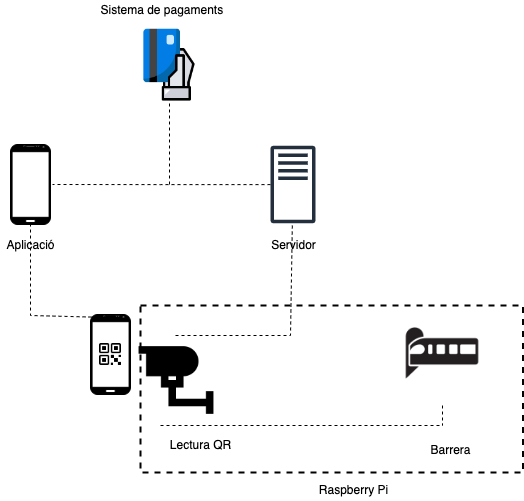
\includegraphics[height=0.85\textheight]{arquitectura_sistema}
    \end{figure}
\end{slide}
\section{Back-end}
\subsection{Bases de Dades}
\begin{slide}
    \begin{figure}[H]
        \centering
        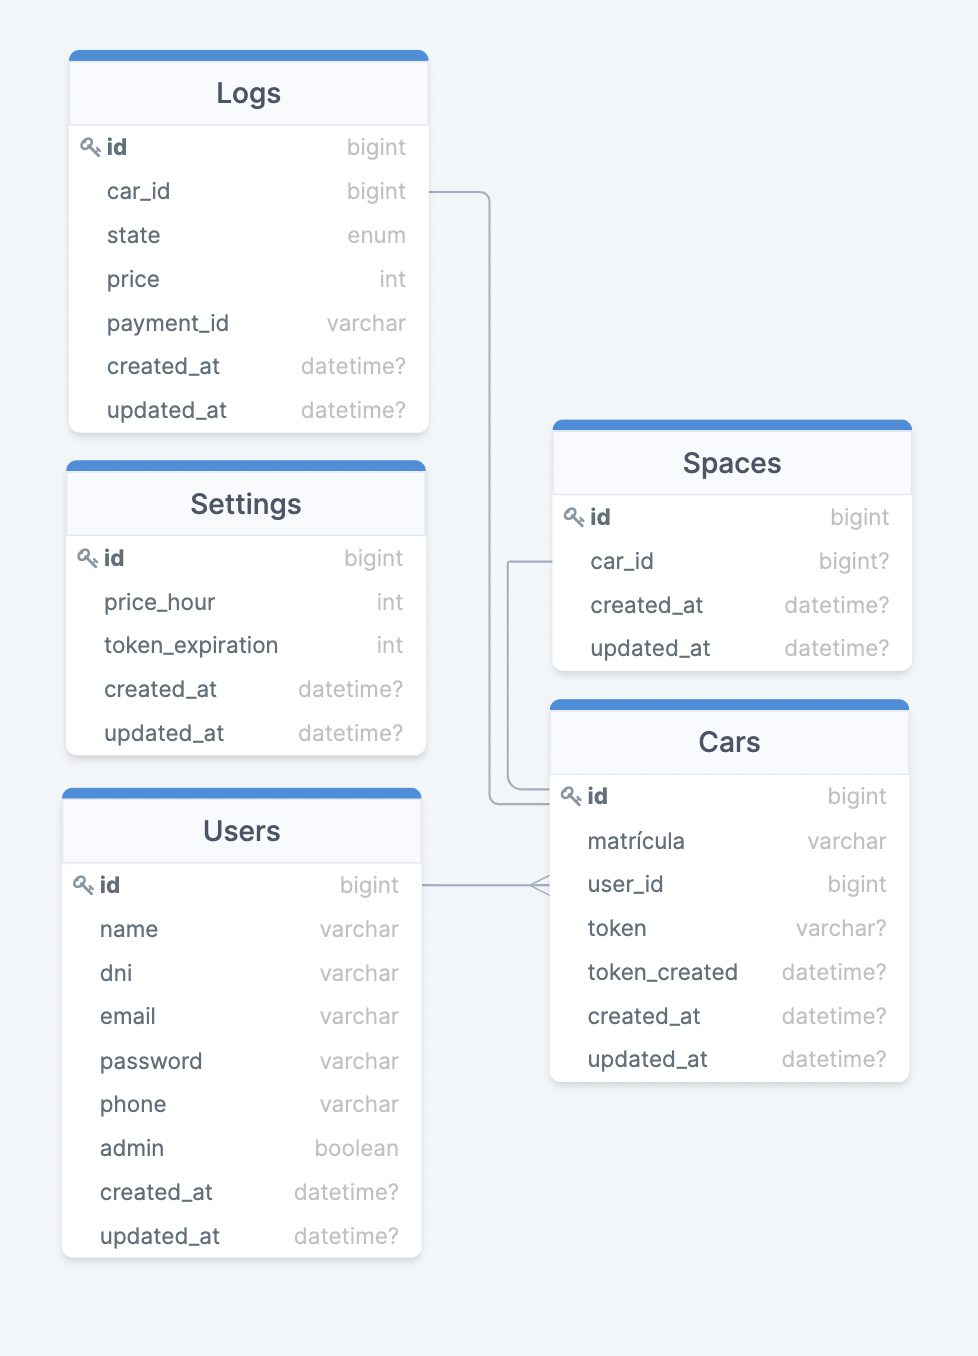
\includegraphics[height=0.95\textheight]{BD}
    \end{figure}
\end{slide}

% \begin{slide}
%     \begin{figure}[H]
%         \centering
%         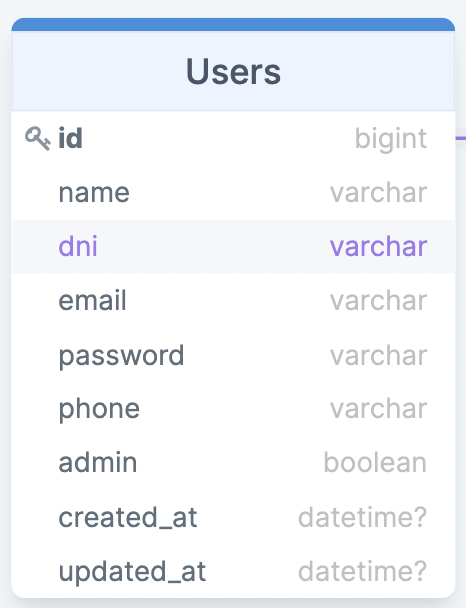
\includegraphics[height=0.35\textheight]{BD_users}
%         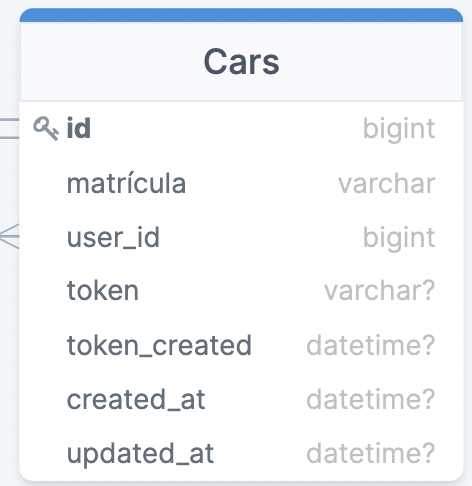
\includegraphics[height=0.35\textheight]{BD_cars}
%         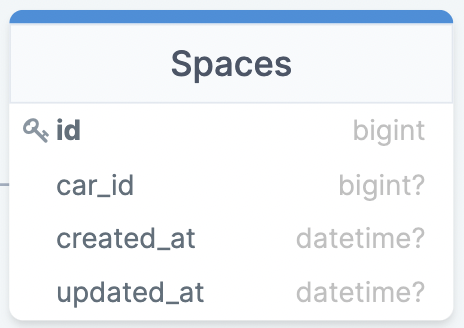
\includegraphics[height=0.35\textheight]{BD_spaces}
%         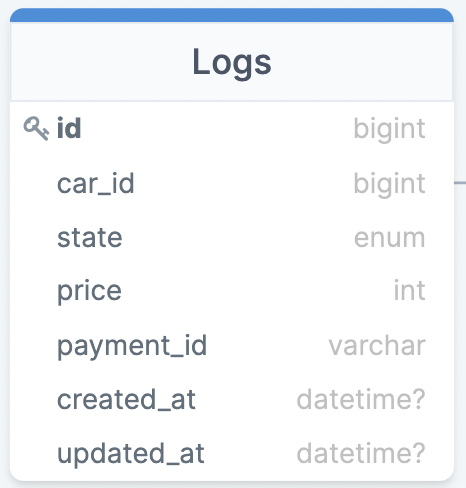
\includegraphics[height=0.35\textheight]{BD_logs}
%         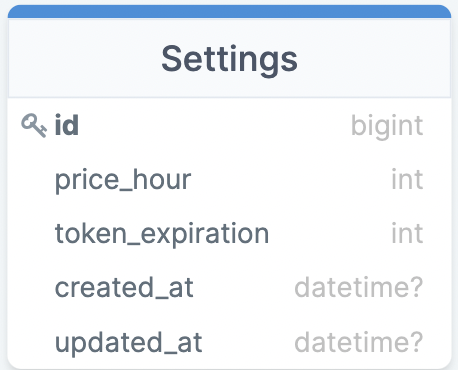
\includegraphics[height=0.35\textheight]{BD_settings}

%     \end{figure}
% \end{slide}
\subsection{Rest API}
\begin{slide}
    \begin{table}[H]
    \centering
    \begin{tabular}{llll}
        \hline
        \textbf{Mètode} & \textbf{Ruta} & \textbf{Middelware} & \textbf{Descripció} \\ \hline
        POST            & /auth/login     & guest &  Iniciar sessió     \\ \hline
        POST            & /auth/logout    & guest &  Tancar sessió     \\ \hline
        POST            & /auth/register  & auth  &  Crear usuari    \\ \hline
        GET             & /auth/user      & auth  &  Obtenir usuari    \\ \hline
        PUT             & /auth/user      & auth  &  Modificar usuari  \\ \hline
        \end{tabular}
    \caption{Taula rest API \emph{Auth}}
    \end{table}
\end{slide}

\begin{slide}
    \begin{table}[H]
    \centering
    \begin{tabular}{llll}
    \hline
    \textbf{Mètode} & \textbf{Ruta} & \textbf{Middelware} & \textbf{Descripció} \\ \hline
        GET             & /cars       & auth &  Mostrar tots els cotxes     \\ \hline
        POST            & /cars        & auth & Crear un cotxe     \\ \hline
        GET             & /cars/\{car\}  & auth & Mostrar el cotxe     \\ \hline
        PUT             & /cars/\{car\}  & auth & Modificar el cotxe     \\ \hline
        DELETE          & /cars/\{car\}  & auth & Eliminar el cotxe     \\ \hline
        \end{tabular}
    \caption{Taula rest API \emph{Cars}}
    \end{table}
\end{slide}

\begin{slide}
    \begin{table}[H]
        \centering
        \begin{tabular}{llll}
        \hline
        \textbf{Mètode} & \textbf{Ruta} & \textbf{Middelware} & \textbf{Descripció} \\ \hline
        GET             & /cars/\{car\}/qr   &  auth  & Generar QR  \\ \hline
        \end{tabular}
        \caption{Taula rest API \emph{QR}}
    \end{table}
\end{slide}

\begin{slide}
    \begin{table}[H]
        \centering
        \begin{tabular}{lll}
            \hline
            \textbf{Mètode} & \textbf{Ruta} & \textbf{Descripció} \\ \hline
            POST            & /barriers/open &  Pujar barrera     \\ \hline
        \end{tabular}
        \caption{Taula rest API \emph{Barriers}}
    \end{table}
\end{slide}

\begin{slide}
    \begin{table}[H]
        \centering
        \begin{tabular}{llll}
            \hline
            \textbf{Mètode} & \textbf{Ruta} & \textbf{Middelware} &\textbf{Descripció} \\ \hline
            POST            & /checkout/\{car\}         & auth                & \begin{tabular}[c]{@{}l@{}}Generar \\ pagament\end{tabular}     \\ \hline
            GET             & /checkout/\{car\}/error   & -                   & \begin{tabular}[c]{@{}l@{}}Pagament \\ cancel·lat\end{tabular} \\ \hline
            GET             & /checkout/\{car\}/success & -                   & \begin{tabular}[c]{@{}l@{}}Pagament \\ acceptat\end{tabular}    \\ \hline
        \end{tabular}
        \caption{Taula rest API \emph{Payments}}
    \end{table}
\end{slide}

\begin{slide}
    \begin{table}[H]
        \centering
        \begin{tabular}{llll}
            \hline
            \textbf{Mètode} & \textbf{Ruta} & \textbf{Middelware} & \textbf{Descripció} \\ \hline
            GET             & /settings   & auth & Obtenir settings   \\ \hline
            PUT             & /settings   & auth \& admin & Modificar settings    \\ \hline
        \end{tabular}
        \caption{Taula rest API \emph{Settings}}
    \end{table}
\end{slide}
\section{Front-end}
% \subsection{Pàgines}
% \begin{slide}
        \begin{figure}[H]
        \centering
        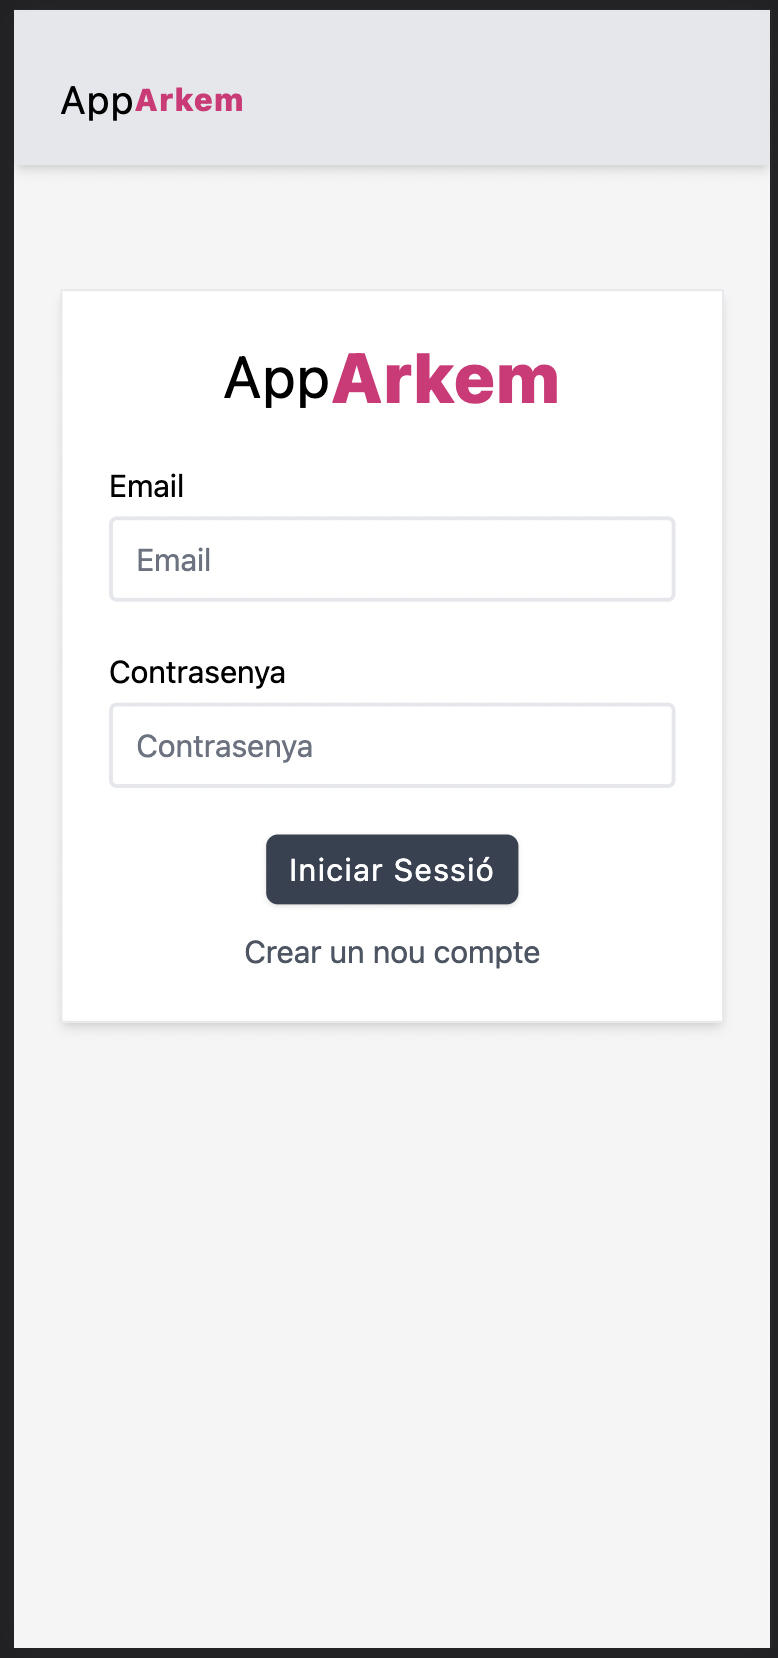
\includegraphics[height=0.60\textheight]{pantalla0_login}
        \caption{Iniciar Sessió}
    \end{figure}
\end{slide}
\begin{slide}
        \begin{figure}[H]
        \centering
        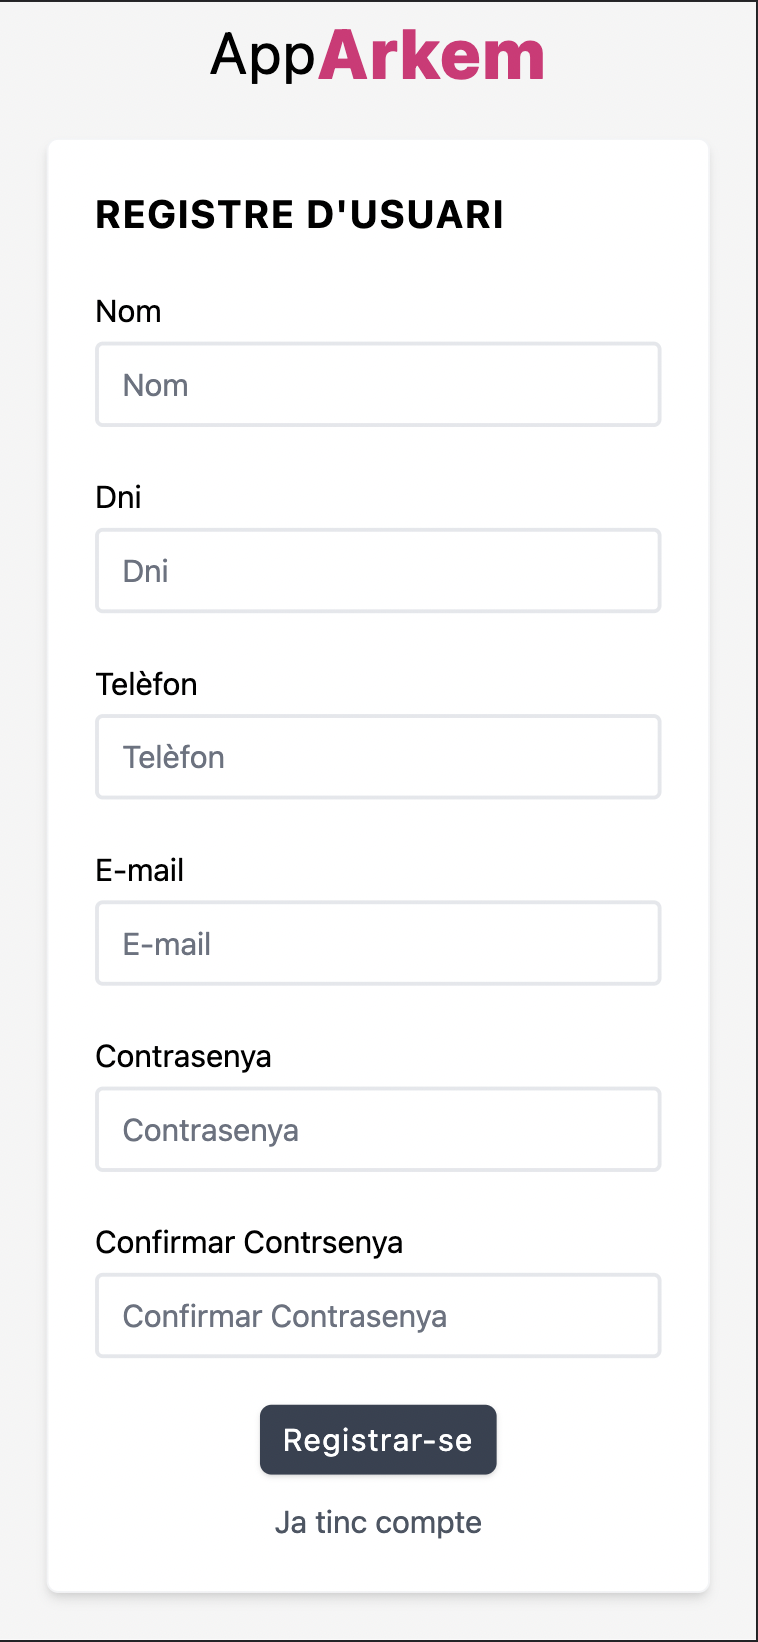
\includegraphics[height=0.60\textheight]{pantalla1_registre}
        \caption{Registre}
    \end{figure}
\end{slide}
\begin{slide}
        \begin{figure}[H]
        \centering
        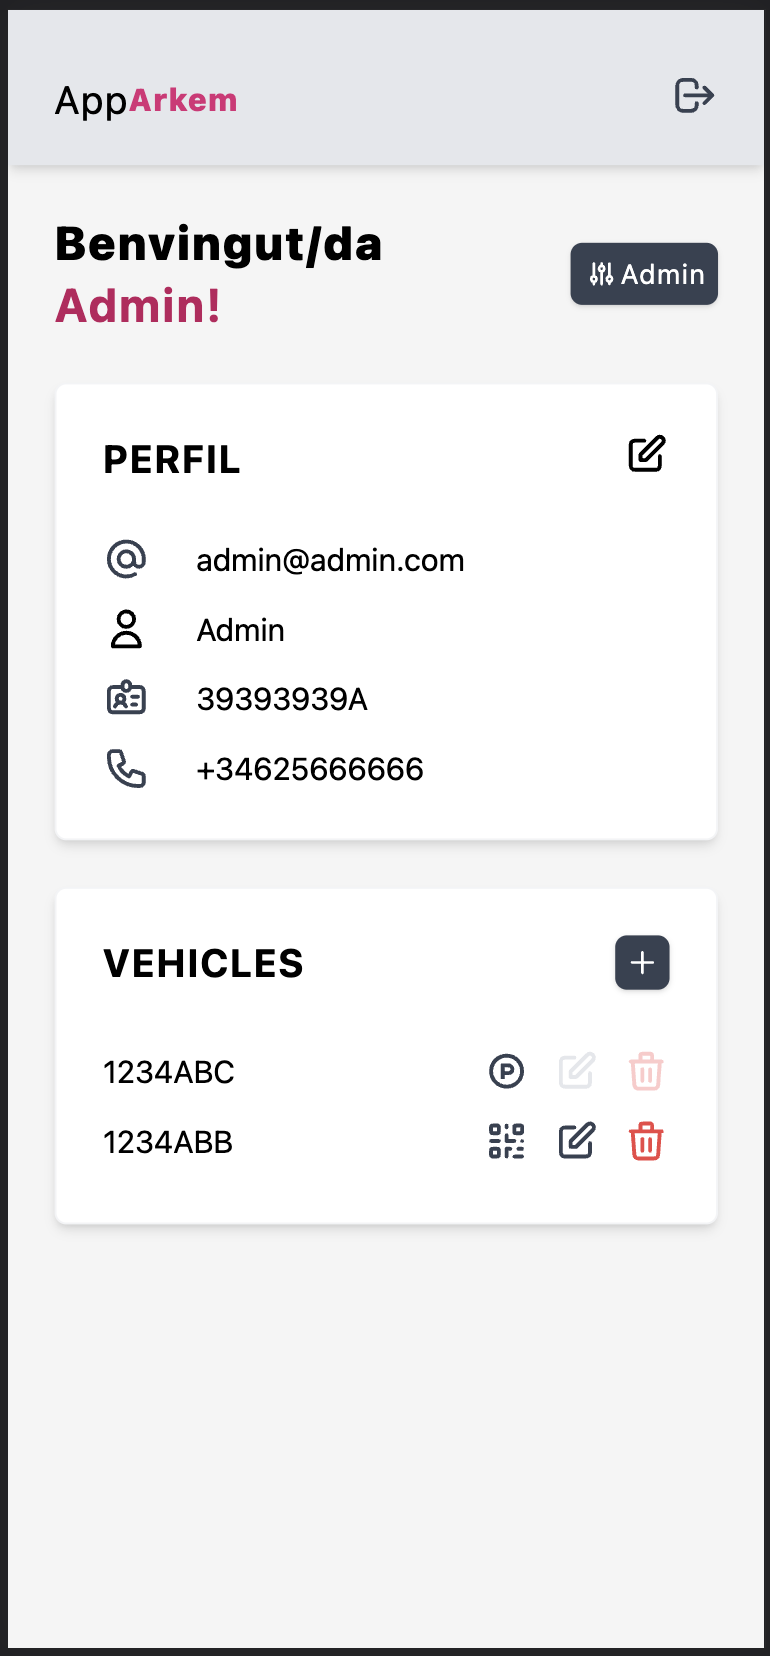
\includegraphics[height=0.60\textheight]{pantalla2_index}
        \caption{Índex}
    \end{figure}
\end{slide}
\begin{slide}
        \begin{figure}[H]
        \centering
        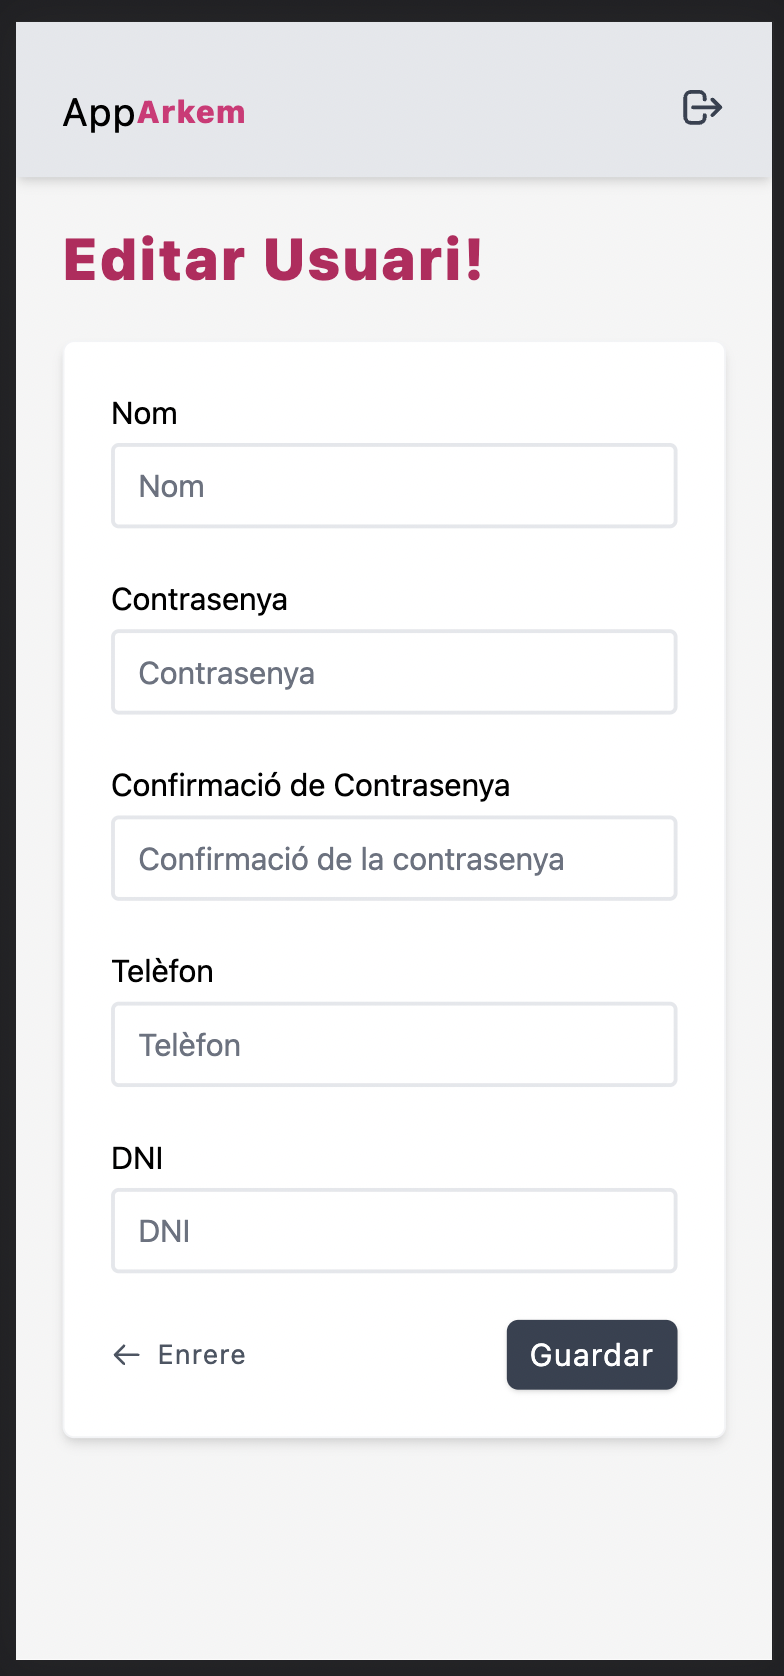
\includegraphics[height=0.60\textheight]{pantalla9_edit_user}
        \caption{Editar usuari}
    \end{figure}
\end{slide}
\begin{slide}
        \begin{figure}[H]
        \centering
        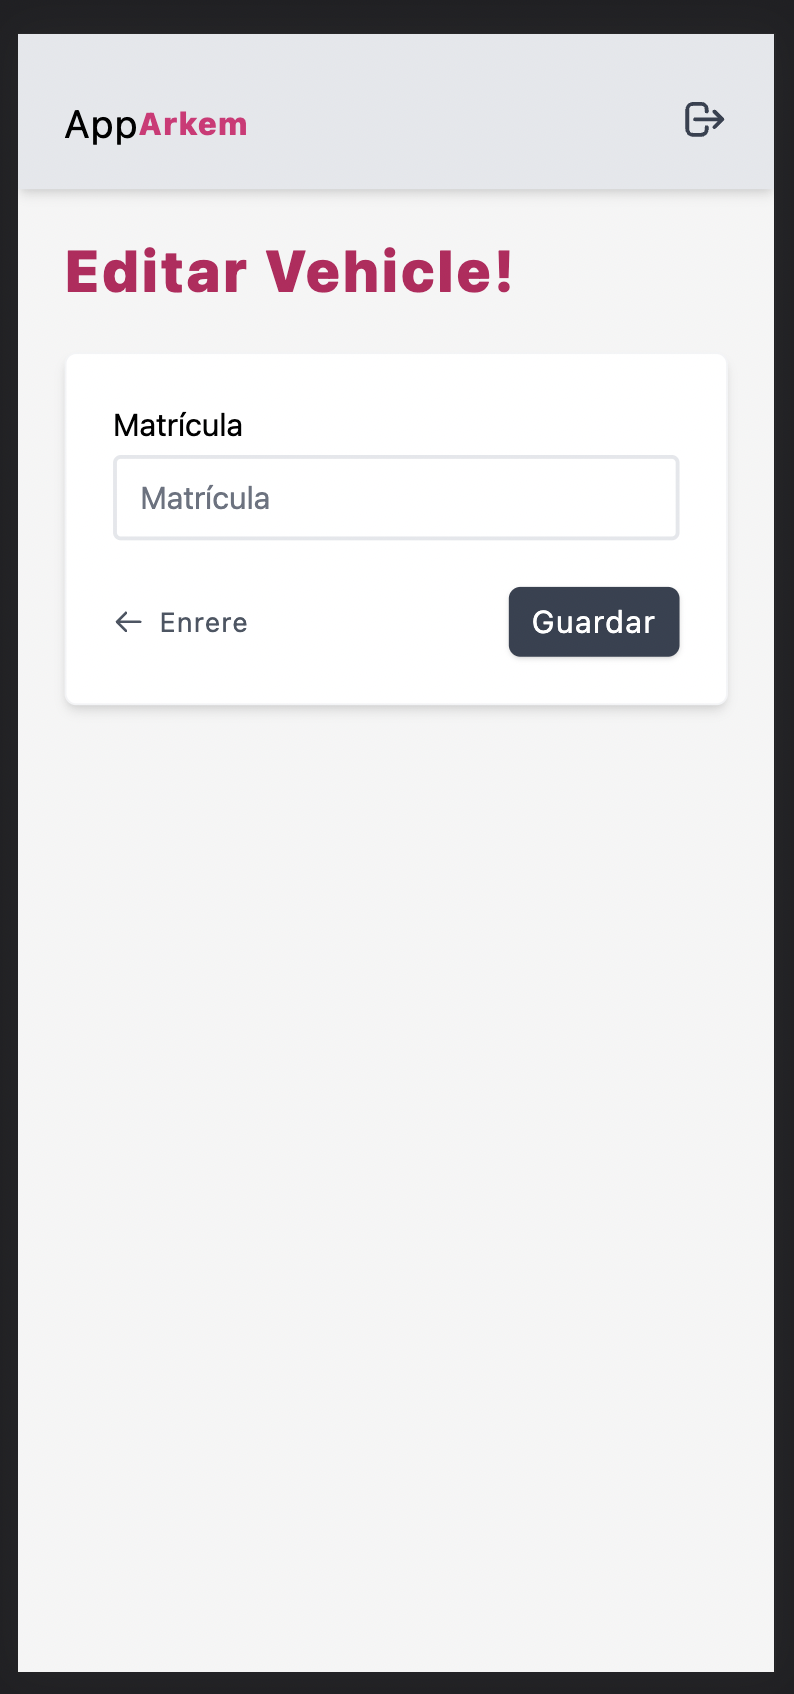
\includegraphics[height=0.60\textheight]{pantalla10_edit_car}
        \caption{Editar vehicle}
    \end{figure}
\end{slide}

% shdsdhsd

\begin{slide}
    \begin{figure}[H]
    \centering
    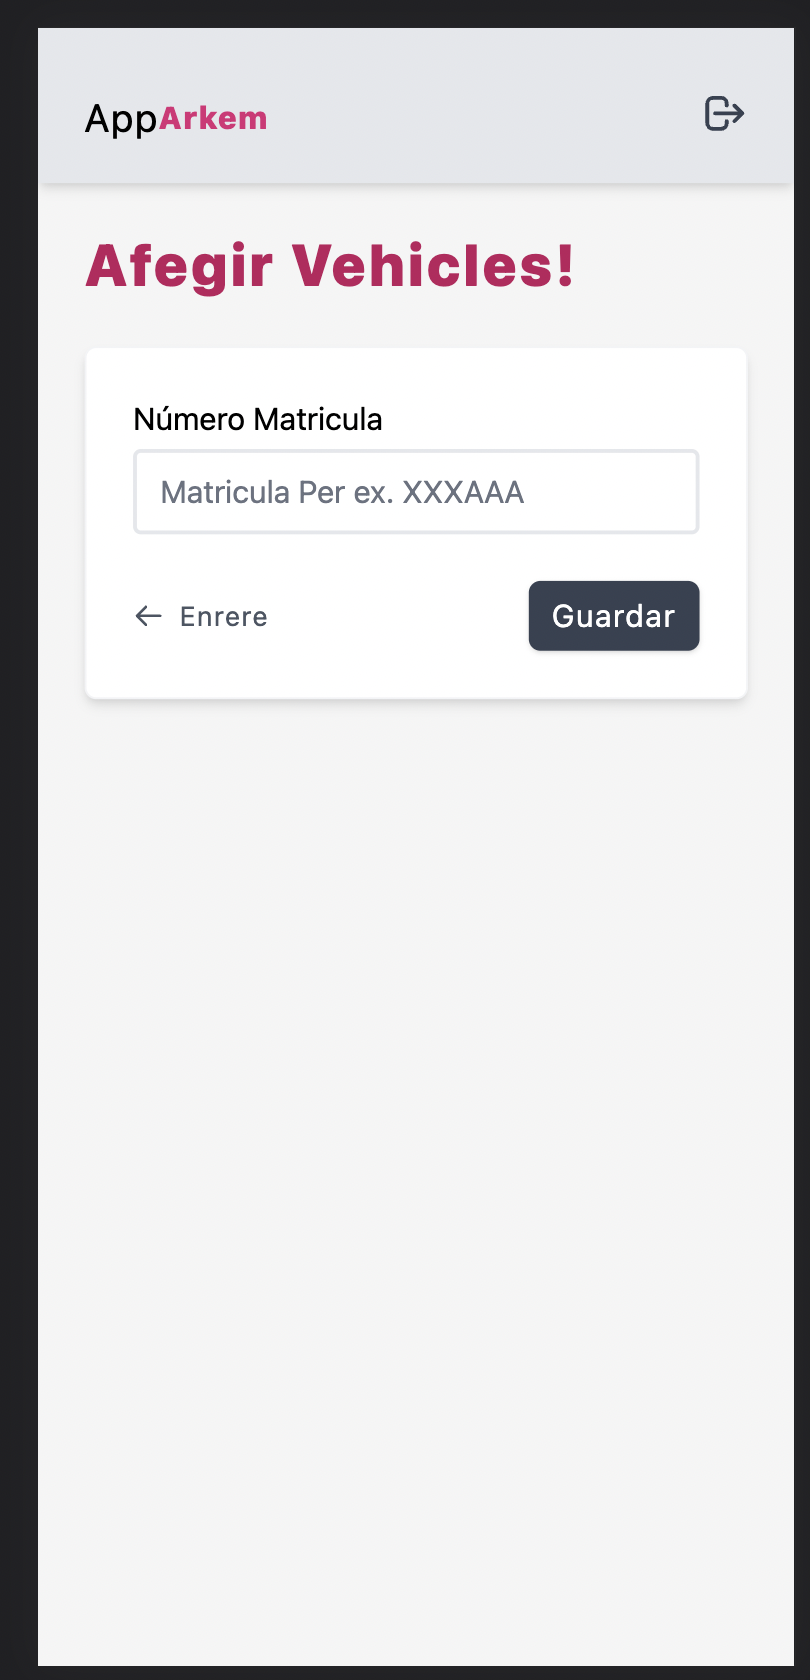
\includegraphics[height=0.60\textheight]{pantalla11_add_car}
    \caption{Afegir cotxes}
\end{figure}
\end{slide}
\begin{slide}
    \begin{figure}[H]
    \centering
    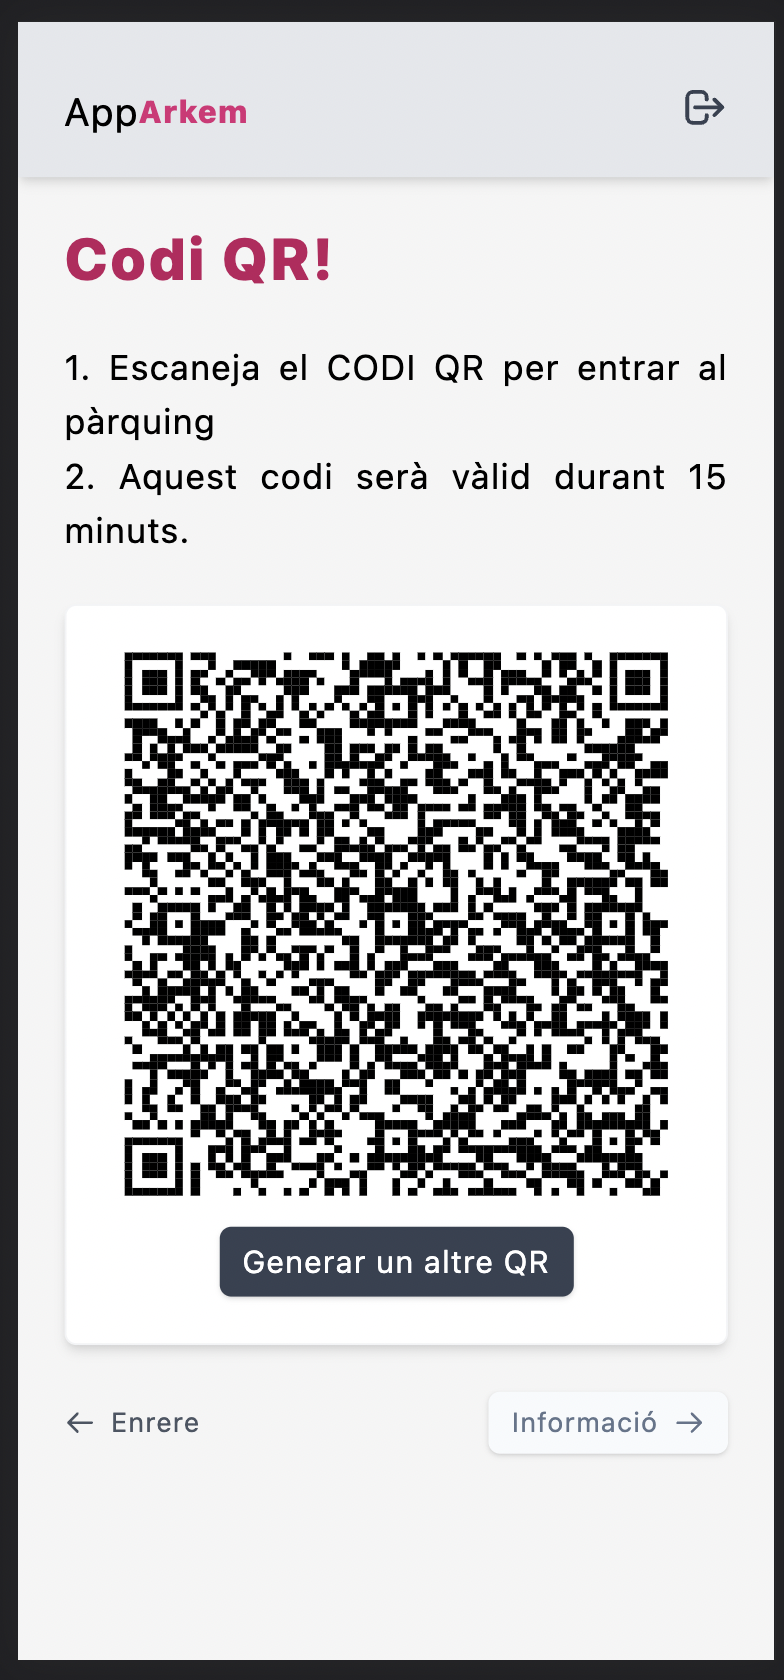
\includegraphics[height=0.60\textheight]{pantalla3_codiQR}
    \caption{Generar codi QR}
\end{figure}
\end{slide}
\begin{slide}
    \begin{figure}[H]
    \centering
    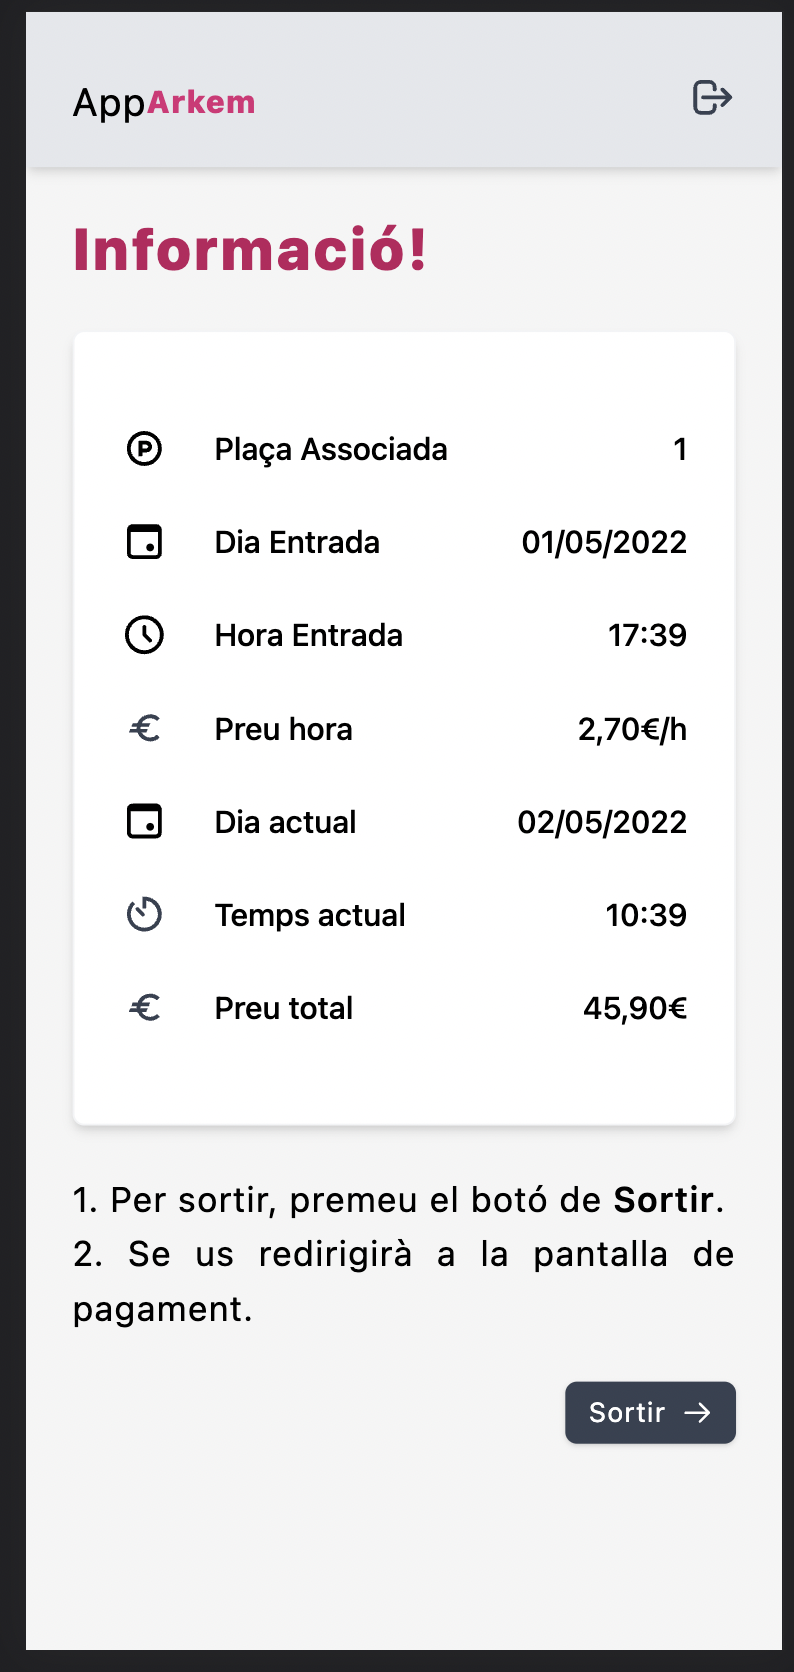
\includegraphics[height=0.60\textheight]{pantalla4_informacio}
    \caption{informació}
\end{figure}
\end{slide}
\begin{slide}
    \begin{figure}[H]
    \centering
    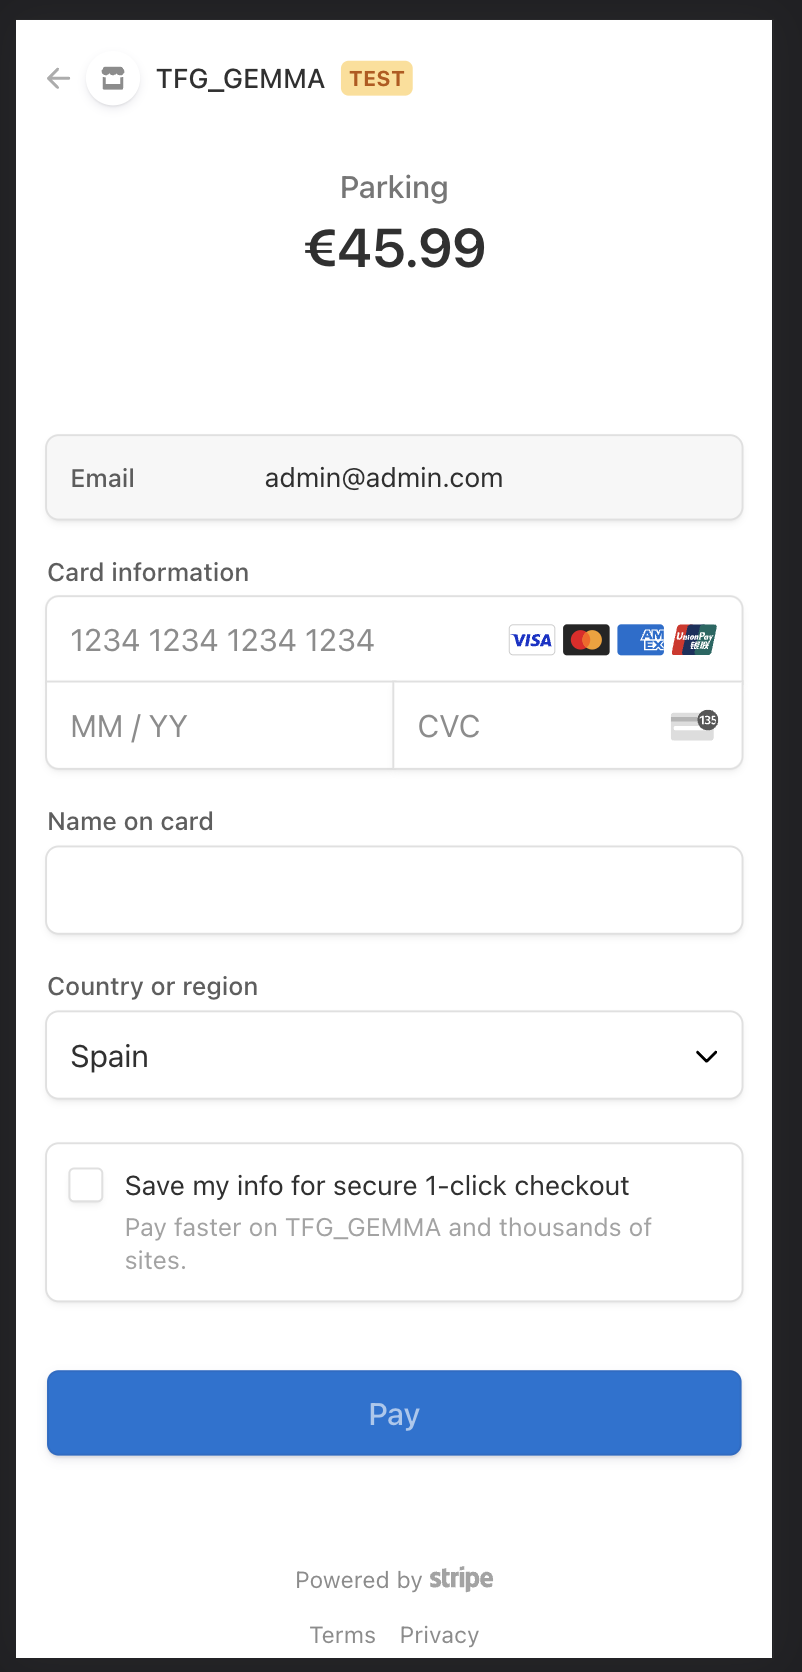
\includegraphics[height=0.60\textheight]{pantalla5_pagament}
    \caption{Pagament d'stripe}
\end{figure}
\end{slide}
\begin{slide}
    \begin{figure}[H]
    \centering
    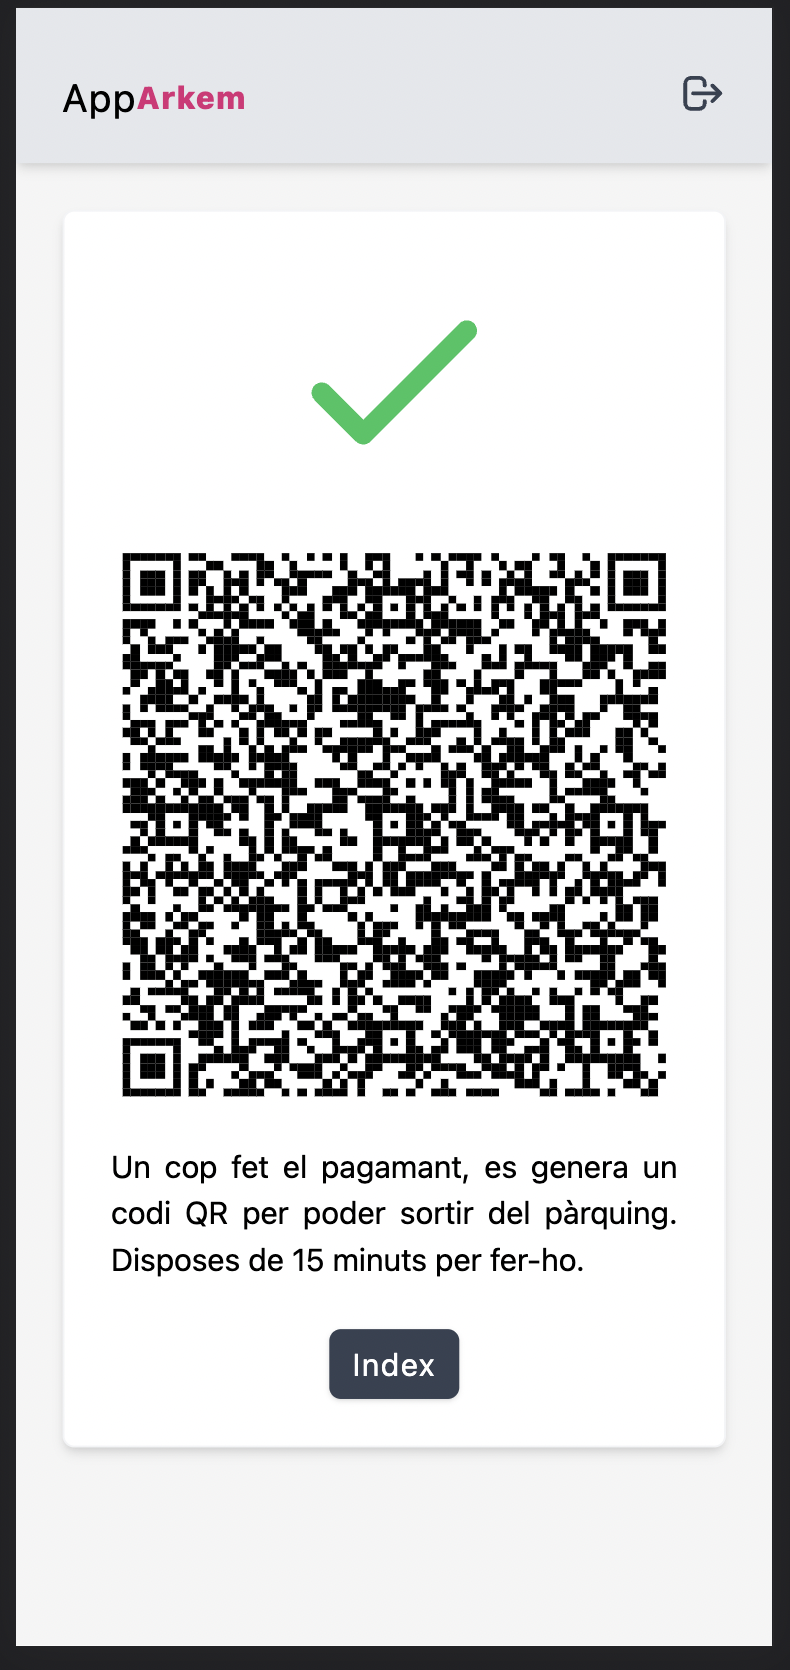
\includegraphics[height=0.60\textheight]{pantalla7_pagament_success}
    \caption{Pagament validat}
\end{figure}
\end{slide}
\begin{slide}
    \begin{figure}[H]
    \centering
    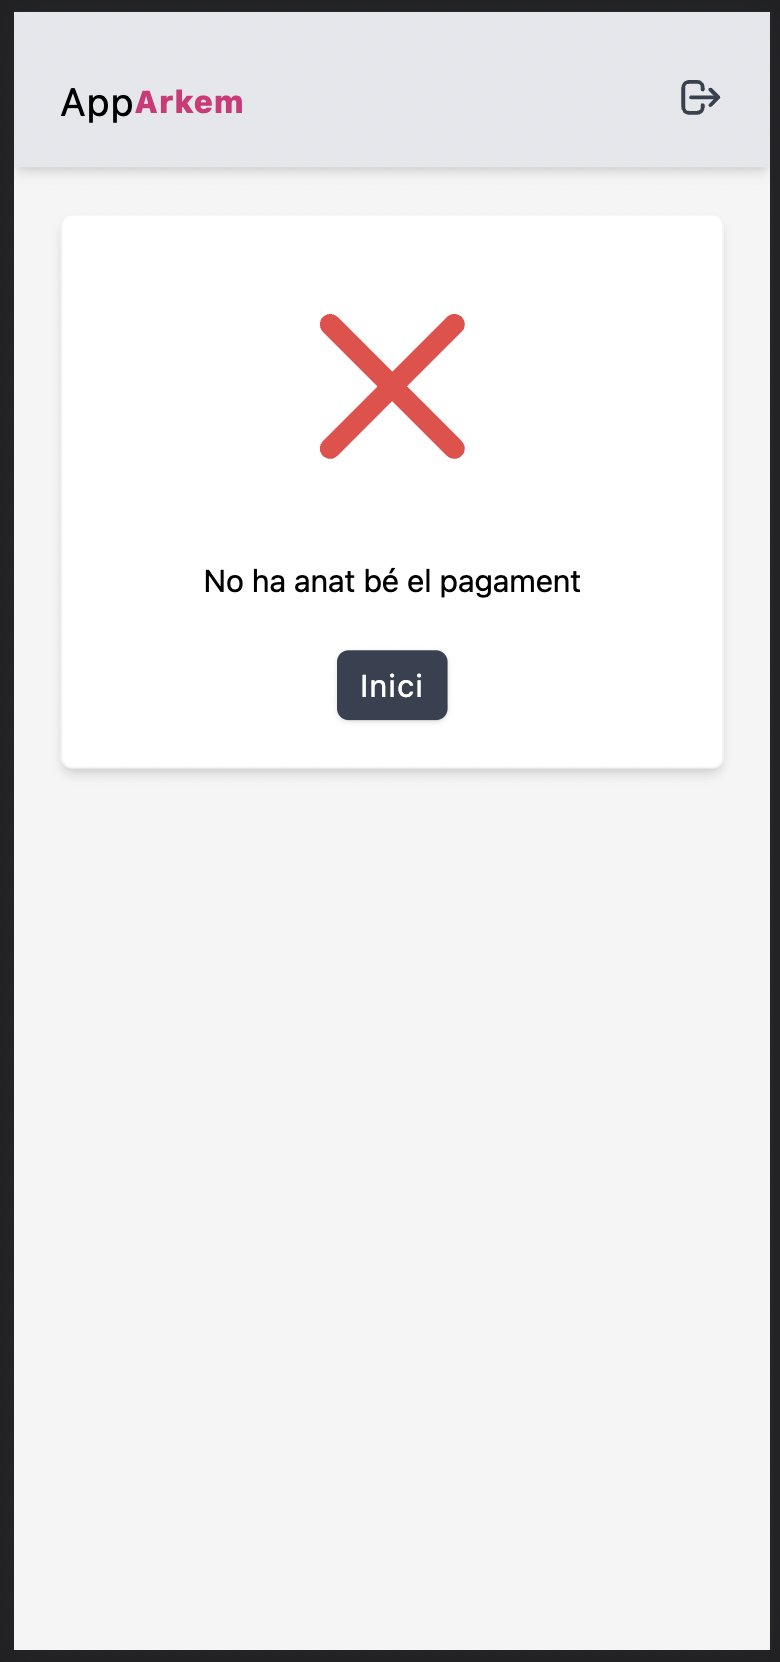
\includegraphics[height=0.60\textheight]{pantalla6_pagamanet_cancel}
    \caption{Pagament cancel·lat}
\end{figure}
\end{slide}
\begin{slide}
    \begin{figure}[H]
    \centering
    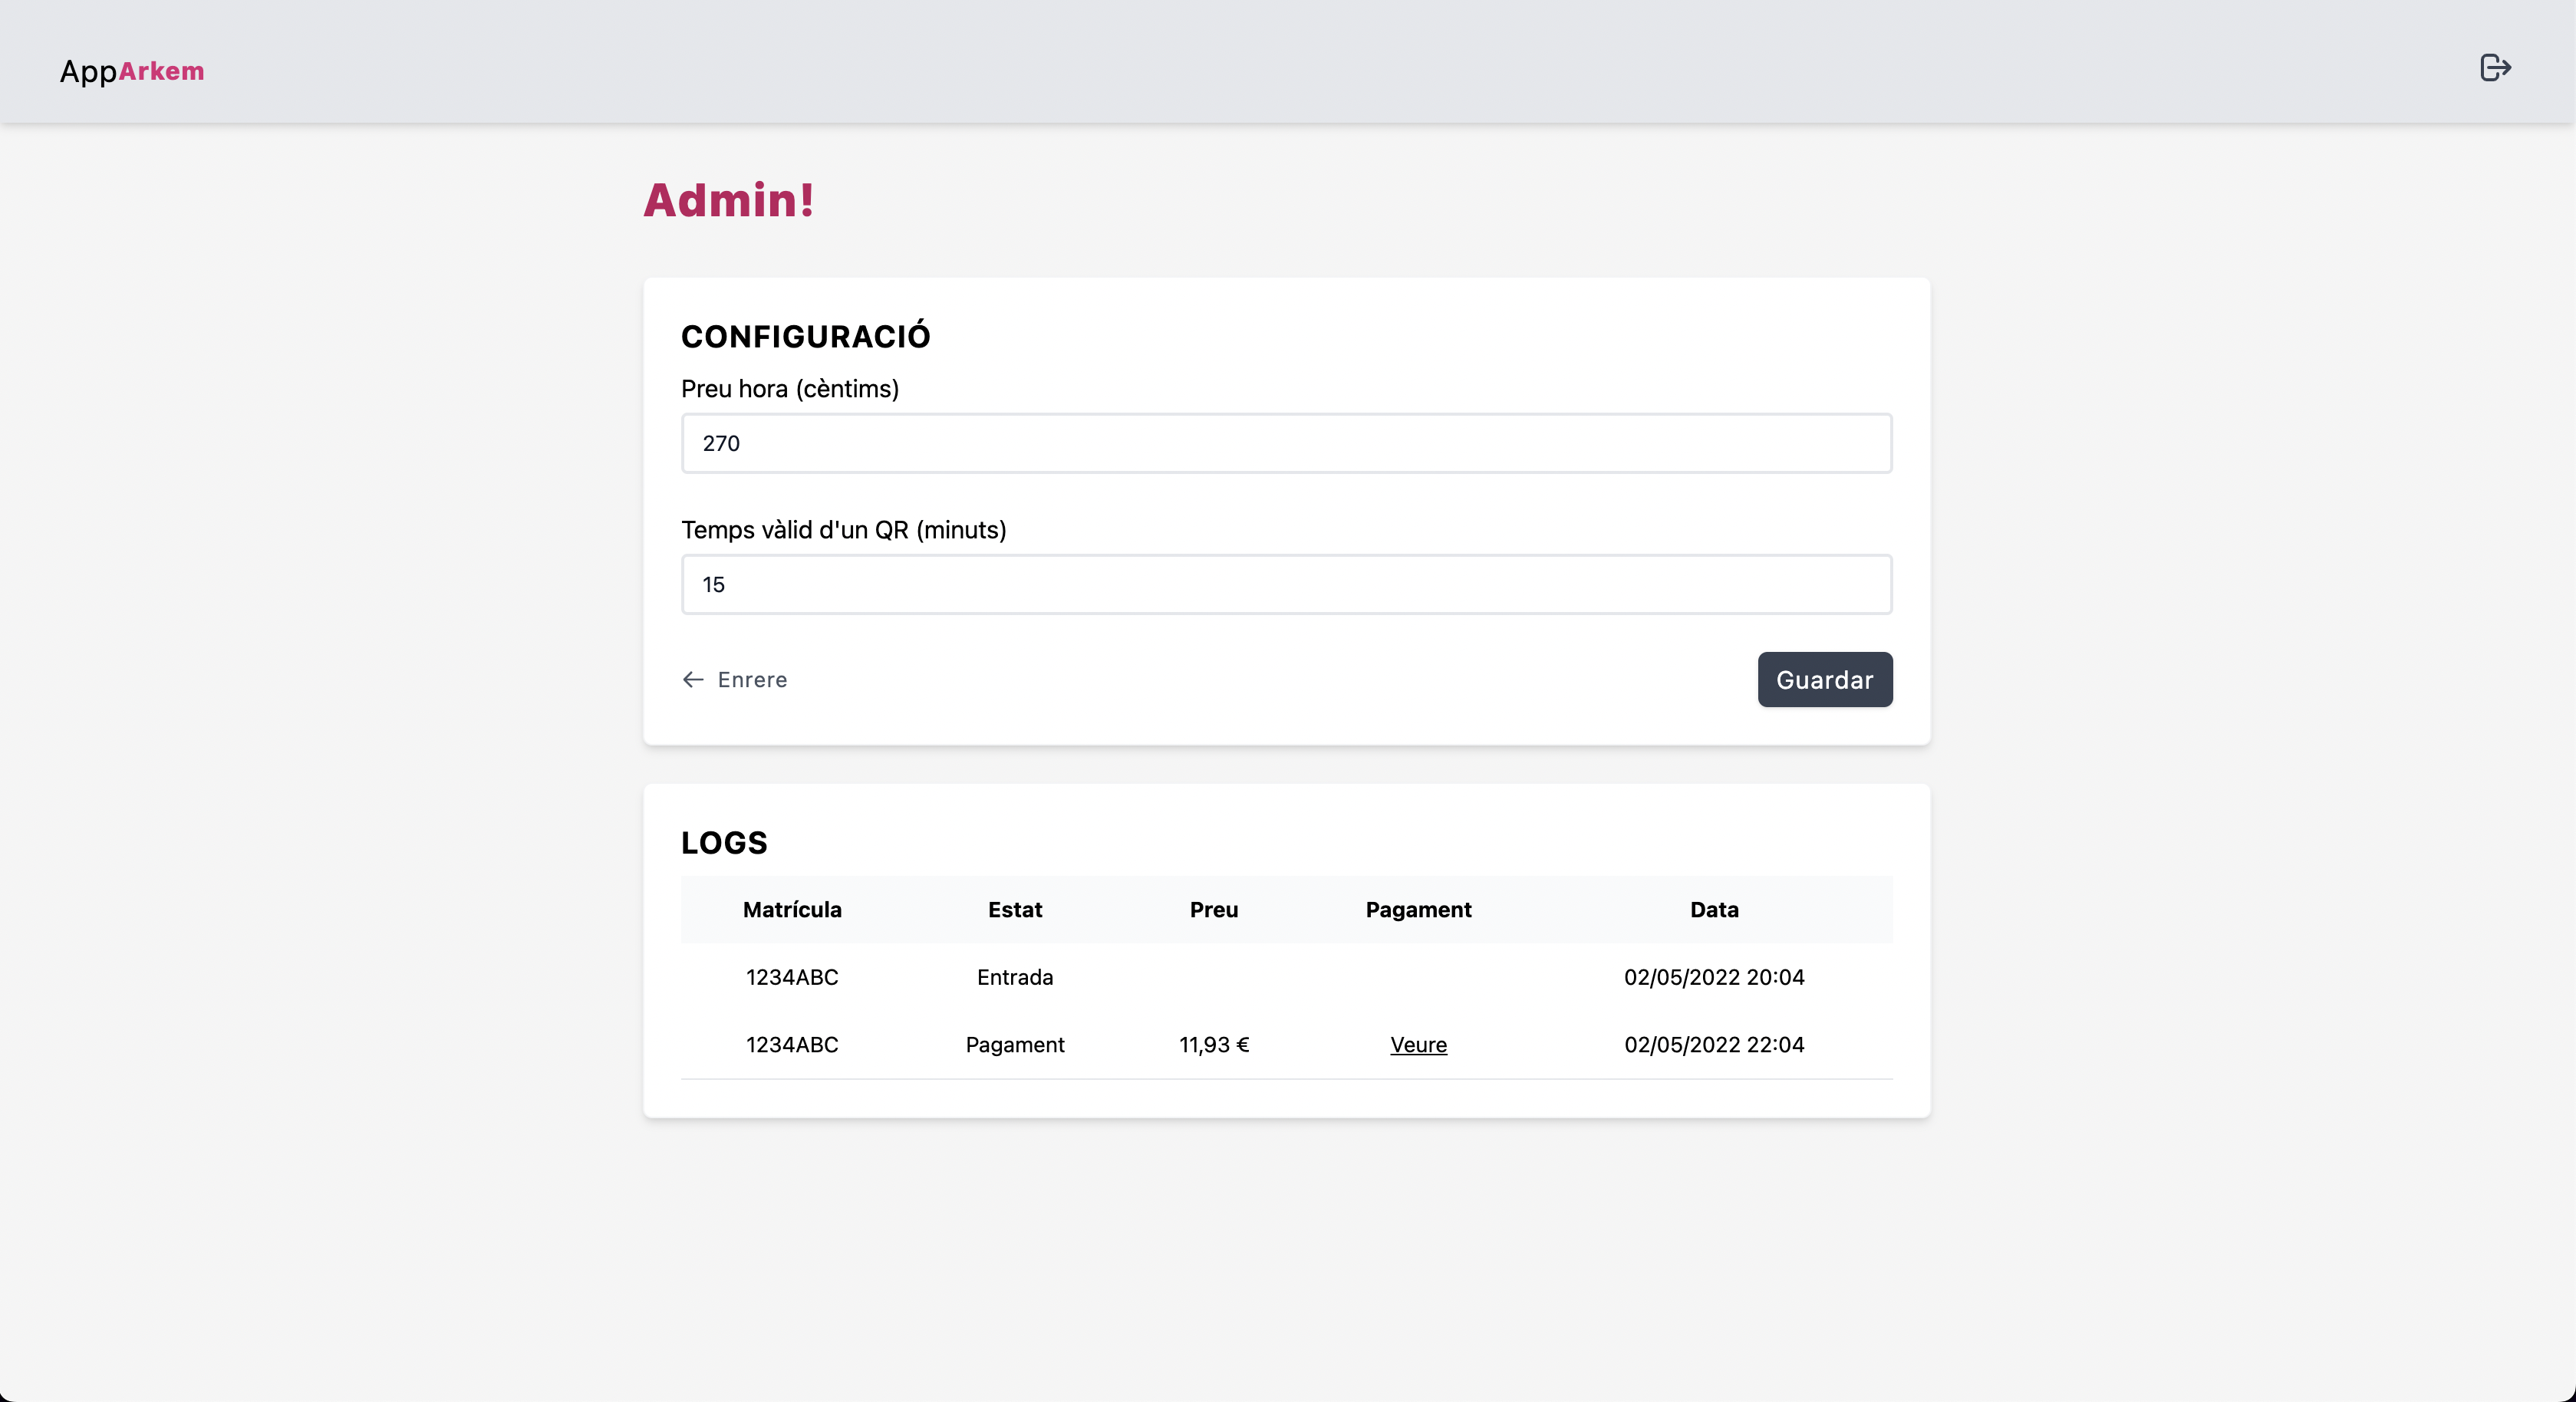
\includegraphics[height=0.70\textheight]{pantalla12_admin}
    \caption{Panell adminstratiu}
\end{figure}
\end{slide}
\begin{slide}
    \begin{figure}[H]
    \centering
    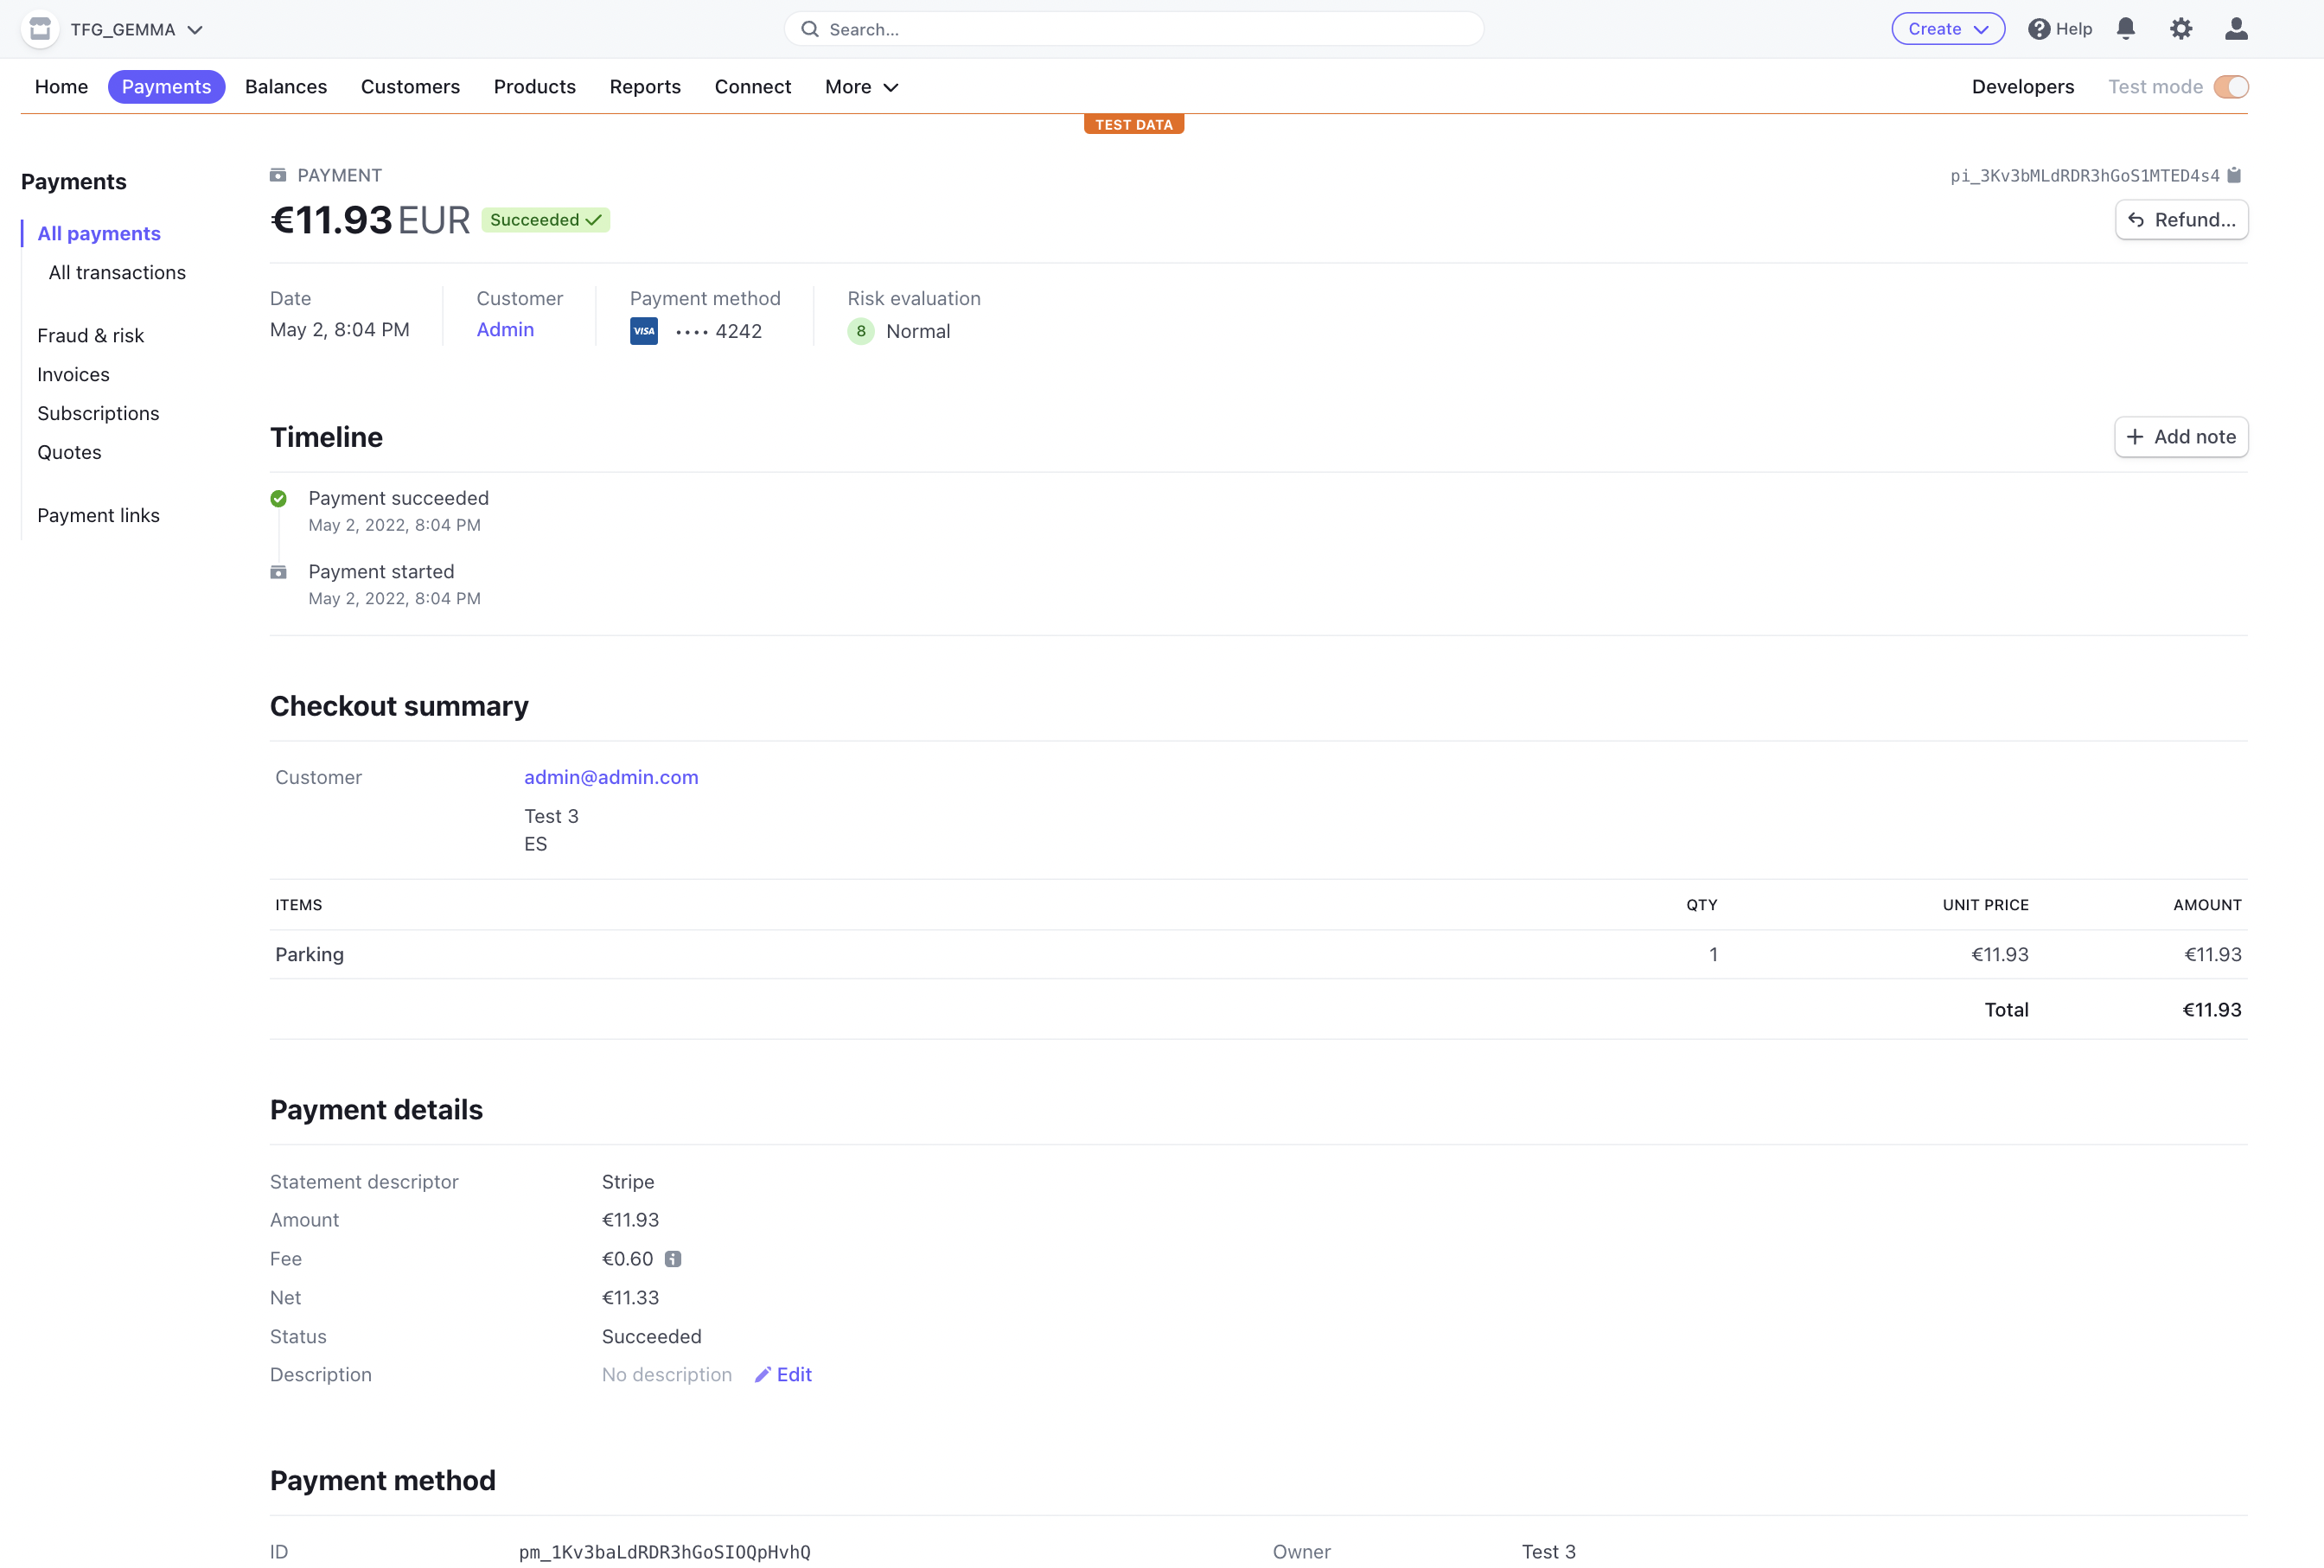
\includegraphics[height=0.70\textheight]{pantalla13_stripe}
    \caption{Vista a Stripe}
\end{figure}
\end{slide}

\section{Raspberry Pi}
\subsection{Barrera}
\begin{slide}
    \begin{figure}[H]
    \centering
        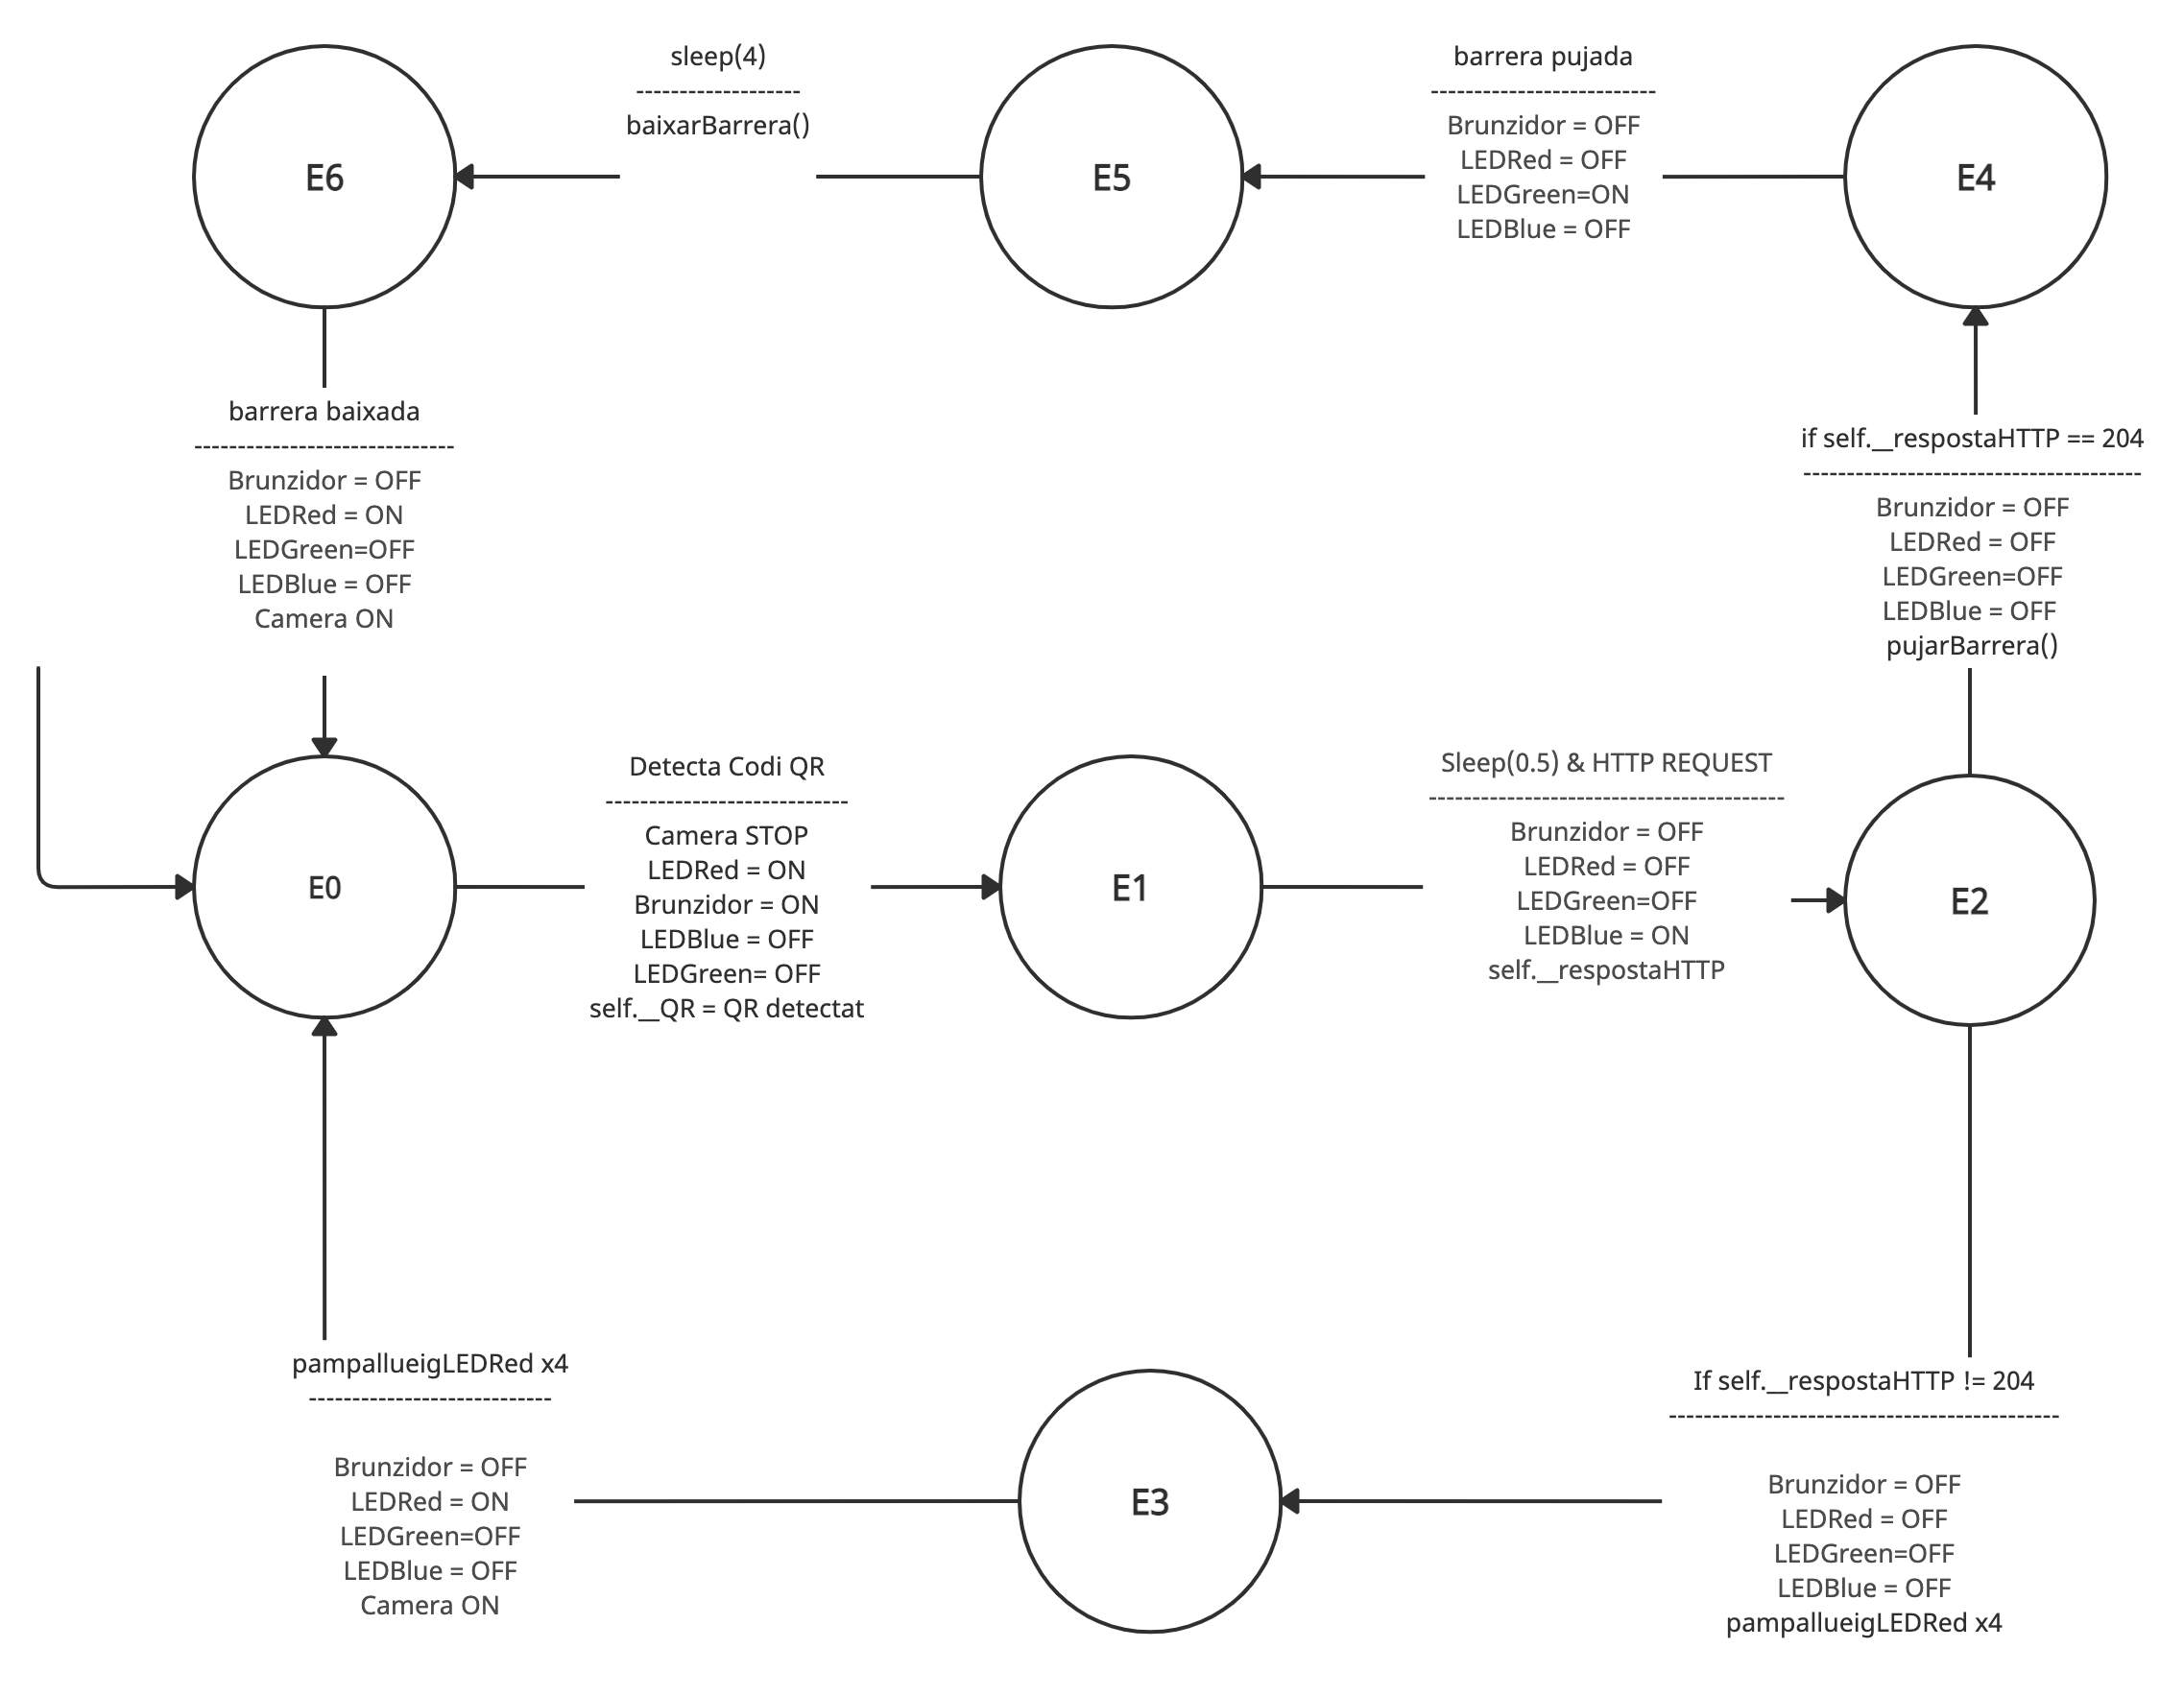
\includegraphics[height=0.85\textheight]{Barrera}
    \end{figure}
\end{slide}
\section{Demostració}
\section{Conclusions}
\subsection{Treball Futur}

Com a treball futur es proposen algunes millores al projecte per tal d'assolir més funcionalitats:

\begin{enumerate}
    \item Afegir o crear un control per part d'administració que pugui pujar o baixar
    la barrera depenent de les necessitats o problemes que puguin succeir. Exceptuant una
    fallada de motor. Per aconseguir aquest efecte és fer que l'actual servidor,
    és a dir, \emph{Laravel} (o \emph{back-end}), passi a ser un client i la Raspberry Pi passi a ser
    un servidor de \emph{Python}. Fer una connexió bidireccional.
    A més a més, crear una taula a la base de dades on es guarda la \emph{ID} i l'estat de la barrera.
    \item Afegir un espai on els usuaris puguin canviar la plaça assignada i puguin
    escollir la plaça desitjada. En l'aplicació fer que els usuaris vegin un mapa
    del pàrquing on pugui seleccionar la plaça, on també mostra les places ocupades
    i lliures en temps real.
    \item Posar la possibilitat de fer reserves de places a través de l'aplicació.
    \item Fins ara, el control d'entrades, sortides i pagaments la veuen els administradors.
    Afegir una pantalla on els clients puguin veure aquesta informació i descarregar-se la factura.
    \item Configurar el servidor de \emph{Laravel} per enviar correus als clients adjuntant la factura
    de cada pagament.
\end{enumerate}

\end{document}